\documentclass[18pts]{article}
\usepackage{amssymb,amsmath,latexsym,enumerate,graphicx,fullpage,url,multicol,longtable,color}
\usepackage{graphicx, tikz}
\usetikzlibrary{calc,shadows}
\usepackage[T1]{fontenc}
\usepackage{eso-pic,fancybox}
\usepackage[absolute,overlay]{textpos}
\usepackage{color}
\usepackage{mathptmx}
\usepackage{fix-cm}

%    \topmargin 0 in
%    \textheight 11in
%    \textwidth 6.25 in
%    \oddsidemargin 1in   % read Lamport p.163
%    \evensidemargin 1 in
%    \headsep = 20pt
\usepackage{anyfontsize}
\usepackage{xparse}
\graphicspath{ {images/} }
% suppresses hyphenation and aligns left
\usepackage[none]{hyphenat}
\raggedright



\newcommand\ProjectName[1]{
{
\fontsize{35}{40}\selectfont
\noindent\textbf{#1}\par
}
\vskip 2mm
\fontsize{20}{25}\selectfont
}

\newenvironment{justified}
{
\tolerance=1
\emergencystretch=\maxdimen
\hyphenpenalty=10000
\hbadness=10000
}


\renewcommand\large{
\noindent\fontsize{16}{19}\selectfont}
\renewcommand\Large{
\noindent\fontsize{18}{20}\selectfont}


%%%%%%%%%%%%%%%%%%%%%%%%%%%%%%%%%%%%%%%%%%%%%%%%%%%%%%
%
%					DO NOT CHANGE ANY ABOVE FORMAT/MACRO
%
%%%%%%%%%%%%%%%%%%%%%%%%%%%%%%%%%%%%%%%%%%%%%%%%%%%%%%
\begin{document}

\ProjectName{Automata and\\ Numeration Systems}
\noindent\textbf{Faculty Mentors: {Philipp Hieronymi \& Erik Walsberg}}
\vskip 2mm
\noindent\textbf{Team Leaders: {Eion Blanchard \& Alexi Block Gorman}}
\vskip 2mm
\noindent\textbf{Scholars: Reed Oei, Eric Ma,  Steve O'Brien, Dagoberto Saenz, Mihika Poddar }\\
\vskip 2mm
\Large

\begin{justified}
%%%%%%%% Too much stuff here, someone delete something here. %%%%%%%%
%%%%%%%% Not sure how much shorter we needed this, but it's somewhat shorter now - Reed %%%%%%%%
  Ostrowski numeration systems are numeration systems based on the continued fraction of irrational numbers.
  Characteristic Sturmian words are infinite balanced binary words which the $n$-th digit of the words can be calculated given $n$ in its Ostrowski representation.
%   Ostrowski numeration systems are numeration system based on the continued fraction of irrational numbers.
%   Characteristic Sturmian words are infinite balanced binary words associated with irrational numbers.
%   For any Sturmian word, there is an automaton that can calculate the $n$-th digit of the word given $n$ in its Ostrowski representation.
%   Sturmian words are Ostrowski-automatic words, meaning there is an automaton that can calculate arbitrary digits of a Sturmian word given an index in its Ostrowski representation.
  We create these automata by expanding on algorithms put forth in Hieronymi and Terry's paper ``Ostrowski Numeration Systems.'' \\
  
  % This computation requires addition and verification automata in Ostrowski numeration system for any continued fraction whose coefficients are all less than some constant, which we generate  by expanding on algorithms put forth in Hieronymi and Terry's paper ``Ostrowski Numeration Systems.'' \\

  The theorem prover Walnut automatically decides logical statements expressed via these automata, allowing us to generalize results from Du, Mousavi, Schaeffer, and Shallit's paper ``Decision Algorithms for Fibonacci-Automatic Words, with Applications to Pattern Avoidance'', such as if characteristic Sturmian words are eventually periodic.

\end{justified}
%\begin{center}
%\includegraphics[height=2in]{images/batteries/1.png}
%\includegraphics[height=2in]{images/batteries/Correlation110.png}
%\end{center}
% \vskip 5mm
\begin{figure}[h]
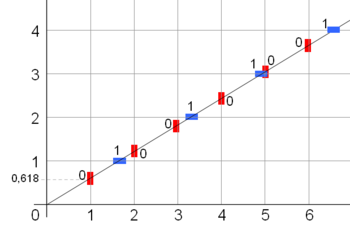
\includegraphics[width=0.49\textwidth]{images/Fibonacci_word_cutting_sequence.png}%
\hfill
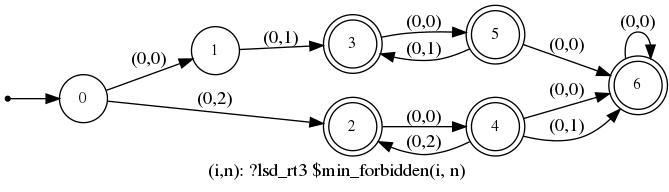
\includegraphics[width=0.49\textwidth]{images/minimal_forbidden_words_rt3.jpg}%
\end{figure}
\end{document} 
